\chapter{Exploratory Data Analysis}
\label{cha:Data analysis}
This chapter starts by describing the dataset were the exploratory data analysis will be performed on in Section \ref{s:Data description}. Next, the preprocessing steps done before the data analysis are explained in Section \ref{s:Preprocessing}. The preprocessing steps consists out of handling missing data, identifying zero days, normalization and removing time series with a big shift in its rolling mean for all the 261 load series with a full year of smart meter measurements. In Section \ref{s:Data Analysis} follows a data analysis on the preprocessed data. For this all the 261 load series with a full year of smart meter measurements are aggregated to identify general characteristics of the data. Things of the aggregated load serie that are assessed are seasonality, comparing electrical consumption between weekdays and weekends, impact of an holiday, the influence of the temperature and the identification of the influence of properties of the household e.g. dwelling type. This last part was possible due to the availability of extra information through a voluntary questionnaire.


\section{Data description}\label{s:Data description}
The data used in this thesis was made available for the \href{https://ieee-dataport.org/competitions/ieee-cis-technical-challenge-energy-prediction-smart-meter-data}{IEEE-CIS technical challenge on energy prediction from smart data}. The dataset consists of load signals with time steps of 30 minutes of 3248 households located in the UK during the year 2017. Only households are considered and no The definition of an household are all the people who occupy a single housing unit, regardless of their relationship to one another. Each smart meter is property of E.ON UK and can collect a maximum  of $17520$ measurements during the year 2017.
 Not all the $3248$ smart meters consist out of full data as can be seen in Figure \ref{fig:amountNaN}. It can be clearly seen that there are $12$ jumps in the amount of missing values. This is because the available data ranges from one month (only December) to a full year of data. This acknowledges that customers may have joined the measuring campaign at different times during the year. There are additional missing values in the time series due to sending or receiving errors of the smart meter.\\
 
 \begin{figure}[h!]
 	\centering
 	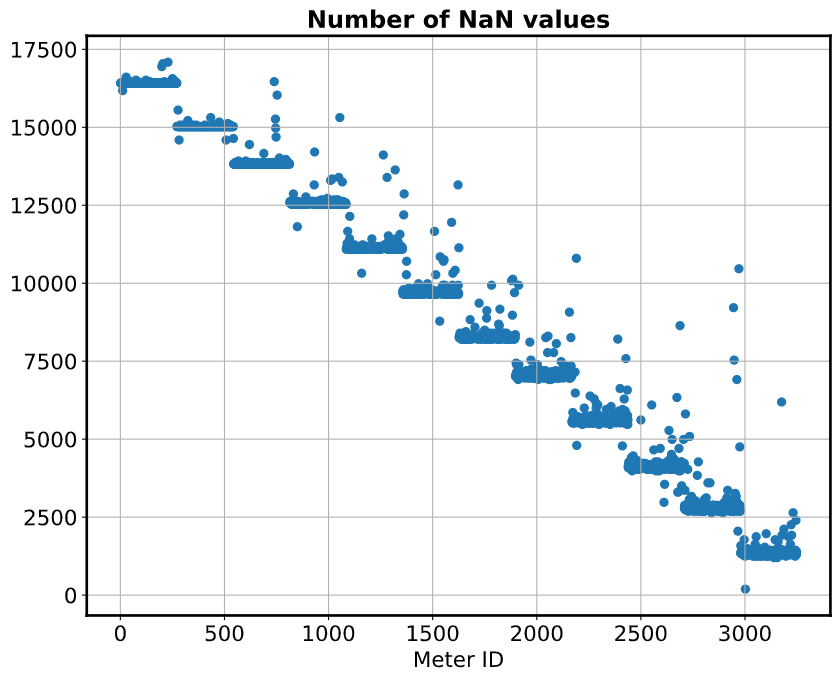
\includegraphics[width=0.8\textwidth]{amountNaN.png}
 	\caption{The amount of NaN values in all the 3248 load signals.}
 	\label{fig:amountNaN}
 \end{figure}

Besides of the electricity consumption of the different households, also information is available about the average, minimum and maximum temperatures on a daily resolution. Finally, extra household information has been partially collected about 2143 households through voluntary surveys. This concerns the dwelling type, number of occupants, number of bedrooms etc. as further detailed in Table \ref{tab:attributes}. From the questionnaire it can be derived that the maximum amount of residents is 4 and there is a maximum amount of bedrooms of 5. The kind of house units are: flat, bungalow, detached house, semi detached house and terraced house. Industrial loads or small businesses e.g. a bakery is not considered. The available datasets and their features are summarized by Table \ref{tab:available_data}.\\

\begin{table}[h]%\[!htb\]	
	\raggedright
	\begin{tabular}[t]{@{}ll}
		\firsthline
		\textbf{Consumption.csv}&\\ \hline
		\# households &3248 \\ 
		Information & Electric load\\
		Max measurements/serie & 17520\\
		Granularity&$ 1/2$ hour\\ 
		Timespan&year 2017 \\    
		Location&UK\\ \bottomrule   
	\end{tabular}
	\hfill
	\raggedleft
	\begin{tabular}[t]{@{}ll}
		\firsthline
		\textbf{Weather.csv}&\\ \hline
		Information & Average temperature\\
		& Max temperature\\
		& Min temperature\\
		Granularity& daily\\ \hline
		\textbf{addInfo.csv}&\\ \hline
		\# households &2143 \\ \bottomrule		    
	\end{tabular}\\
	\caption{Summary of the available csv files form the IEEE-CIS technical challenge.}
	\label{tab:available_data}
\end{table}




\section{Preprocessing}\label{s:Preprocessing}

Following sections describe the preprocessing applied on the 261 load series containing measurements for the entire year. The preprocessing done here is in preparation of the data analysis of Section \ref{s:Data Analysis}. It must not be confused with the preprocessing done for the three considered load series in Chapter \ref{cha:Forecasting the daily electricity consumption}.

\subsection{Missing data} \label{s:missing_data}
As discussed in Section \ref{s:Data description}, there exists two types of missing data in the Consumption csv file as was stated in the data description of the competition: fully missing months, due to the later participation in the measuring campaigns and missing values due to sending or receiving errors of the smart meter. When a smart meter fails, always all the measurements of that day are lost. In this Section two methods to impute the missing values are compared. Method Average Neighbours: replaces a missing value by the mean of the consumption values at the same moment on the next and previous days. Method Mean: substitutes the missing values of a time serie by the mean of all the measurements done by the meter. If the next or previous day is also missing in the serie, two days forward or back in time are used to replace the unknown day and so on. The resulting imputed signals can be seen in Figure \ref{fig:missing_values_imputing}. \\

\begin{figure}[h]
	\begin{subfigure}{0.5\textwidth}
		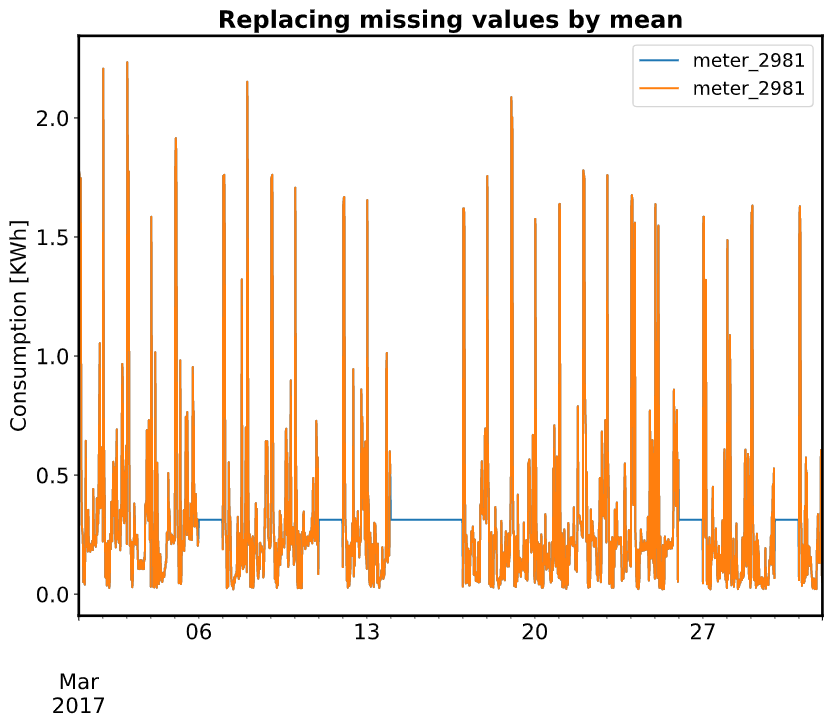
\includegraphics[width=1\linewidth]{mv_mean.png}
		\caption{Mean}
	\end{subfigure}	
	\begin{subfigure}{0.5\textwidth}
		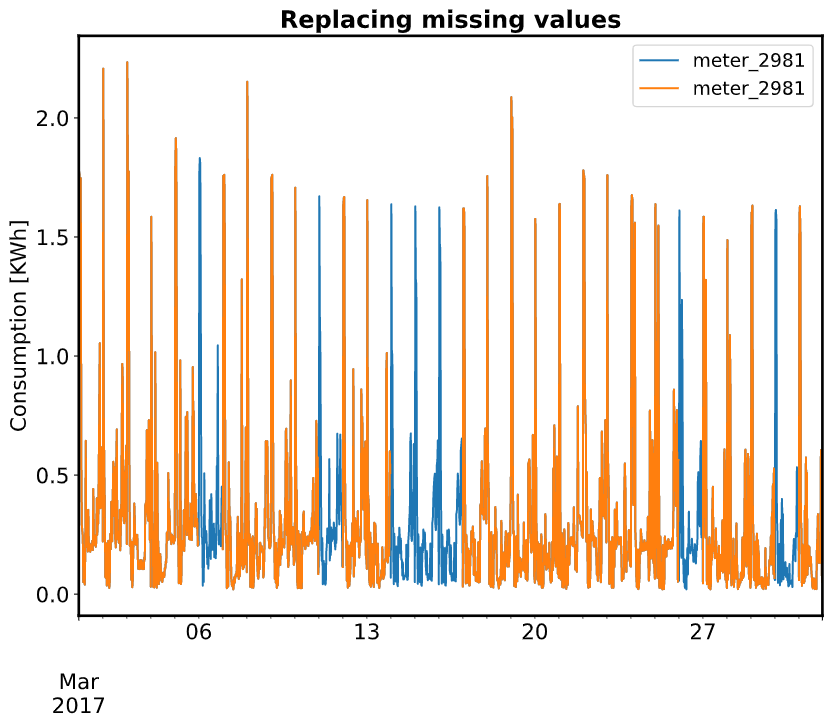
\includegraphics[width=1\linewidth]{mv_s.png}
		\caption{Average Neighbours}
	\end{subfigure}
	\caption{Resulting time serie of the month March after imputation of the missing data.}
	\label{fig:missing_values_imputing}
\end{figure}

In order to compare how accurate both methods impute missing values, 181 months of March without any missing values were used and in each month randomly 7 days were removed. After applying both imputation methods, the resulting estimated signal was compared with the original one and an error value between both signals is calculated, using the mean squared error metric. Normalization is done by dividing the calculated MSE's by the MSE of the worst performing method to calculate the percentage of improvement of one method in comparison to the other. Figure \ref{fig:mv_result} shows that on average, a reduction of the MSE of more then $ 20\% $ is achieved when the average neighbours method is used in comparison to the mean method. Therefore, the average neighbours method will be applied to impute the missing values of the 261 time series with a full year of smart meter measurements. The only exception is made when the first of January and thirty-one December are imputed. Because not both neighbouring days can be known, the mean method is used.

\begin{figure}[h!]
	\centering
	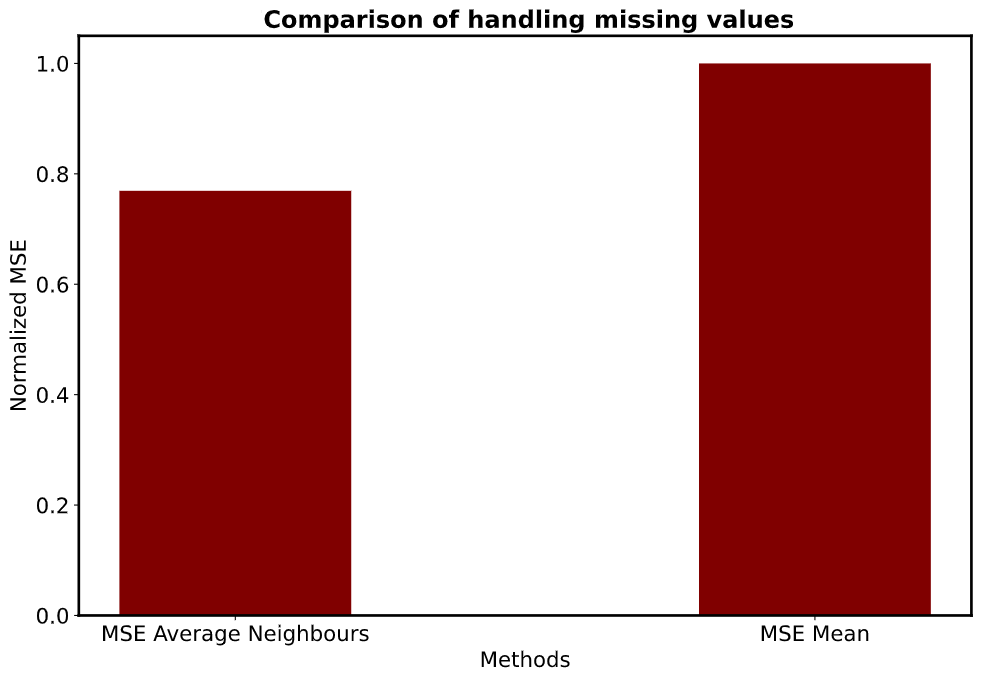
\includegraphics[width=0.8\textwidth]{mv_result.png}
	\caption{Resulting month of March after substitution of the missing values by the mean value of the measurements. }
	\label{fig:mv_result}
\end{figure}

%Actually, used the missing values a bit at random. First imputed the missing values using the average neighbours method and later during the forecasting phase, used different imputation techniques that were not compared with the initial imputation techniques.


\subsection{Zero days}

When inspecting the load series, some untraditional meter measurements were identified. There were $ 9 $ meters of the 261 that had more than one day with a total electrical consumption of zero. Because it is unlikely that a household produces exactly zero kWh on an entire day all these $ 9 $ meters were removed. One of 9 load series is compared in Figure \ref{fig:zero_con} with a load serie with zero days and it is clear that the horizontal lines are not part of a normal household load signal.

\begin{figure}[ht]
	\begin{subfigure}{0.49\textwidth}
		\vspace{4mm}
		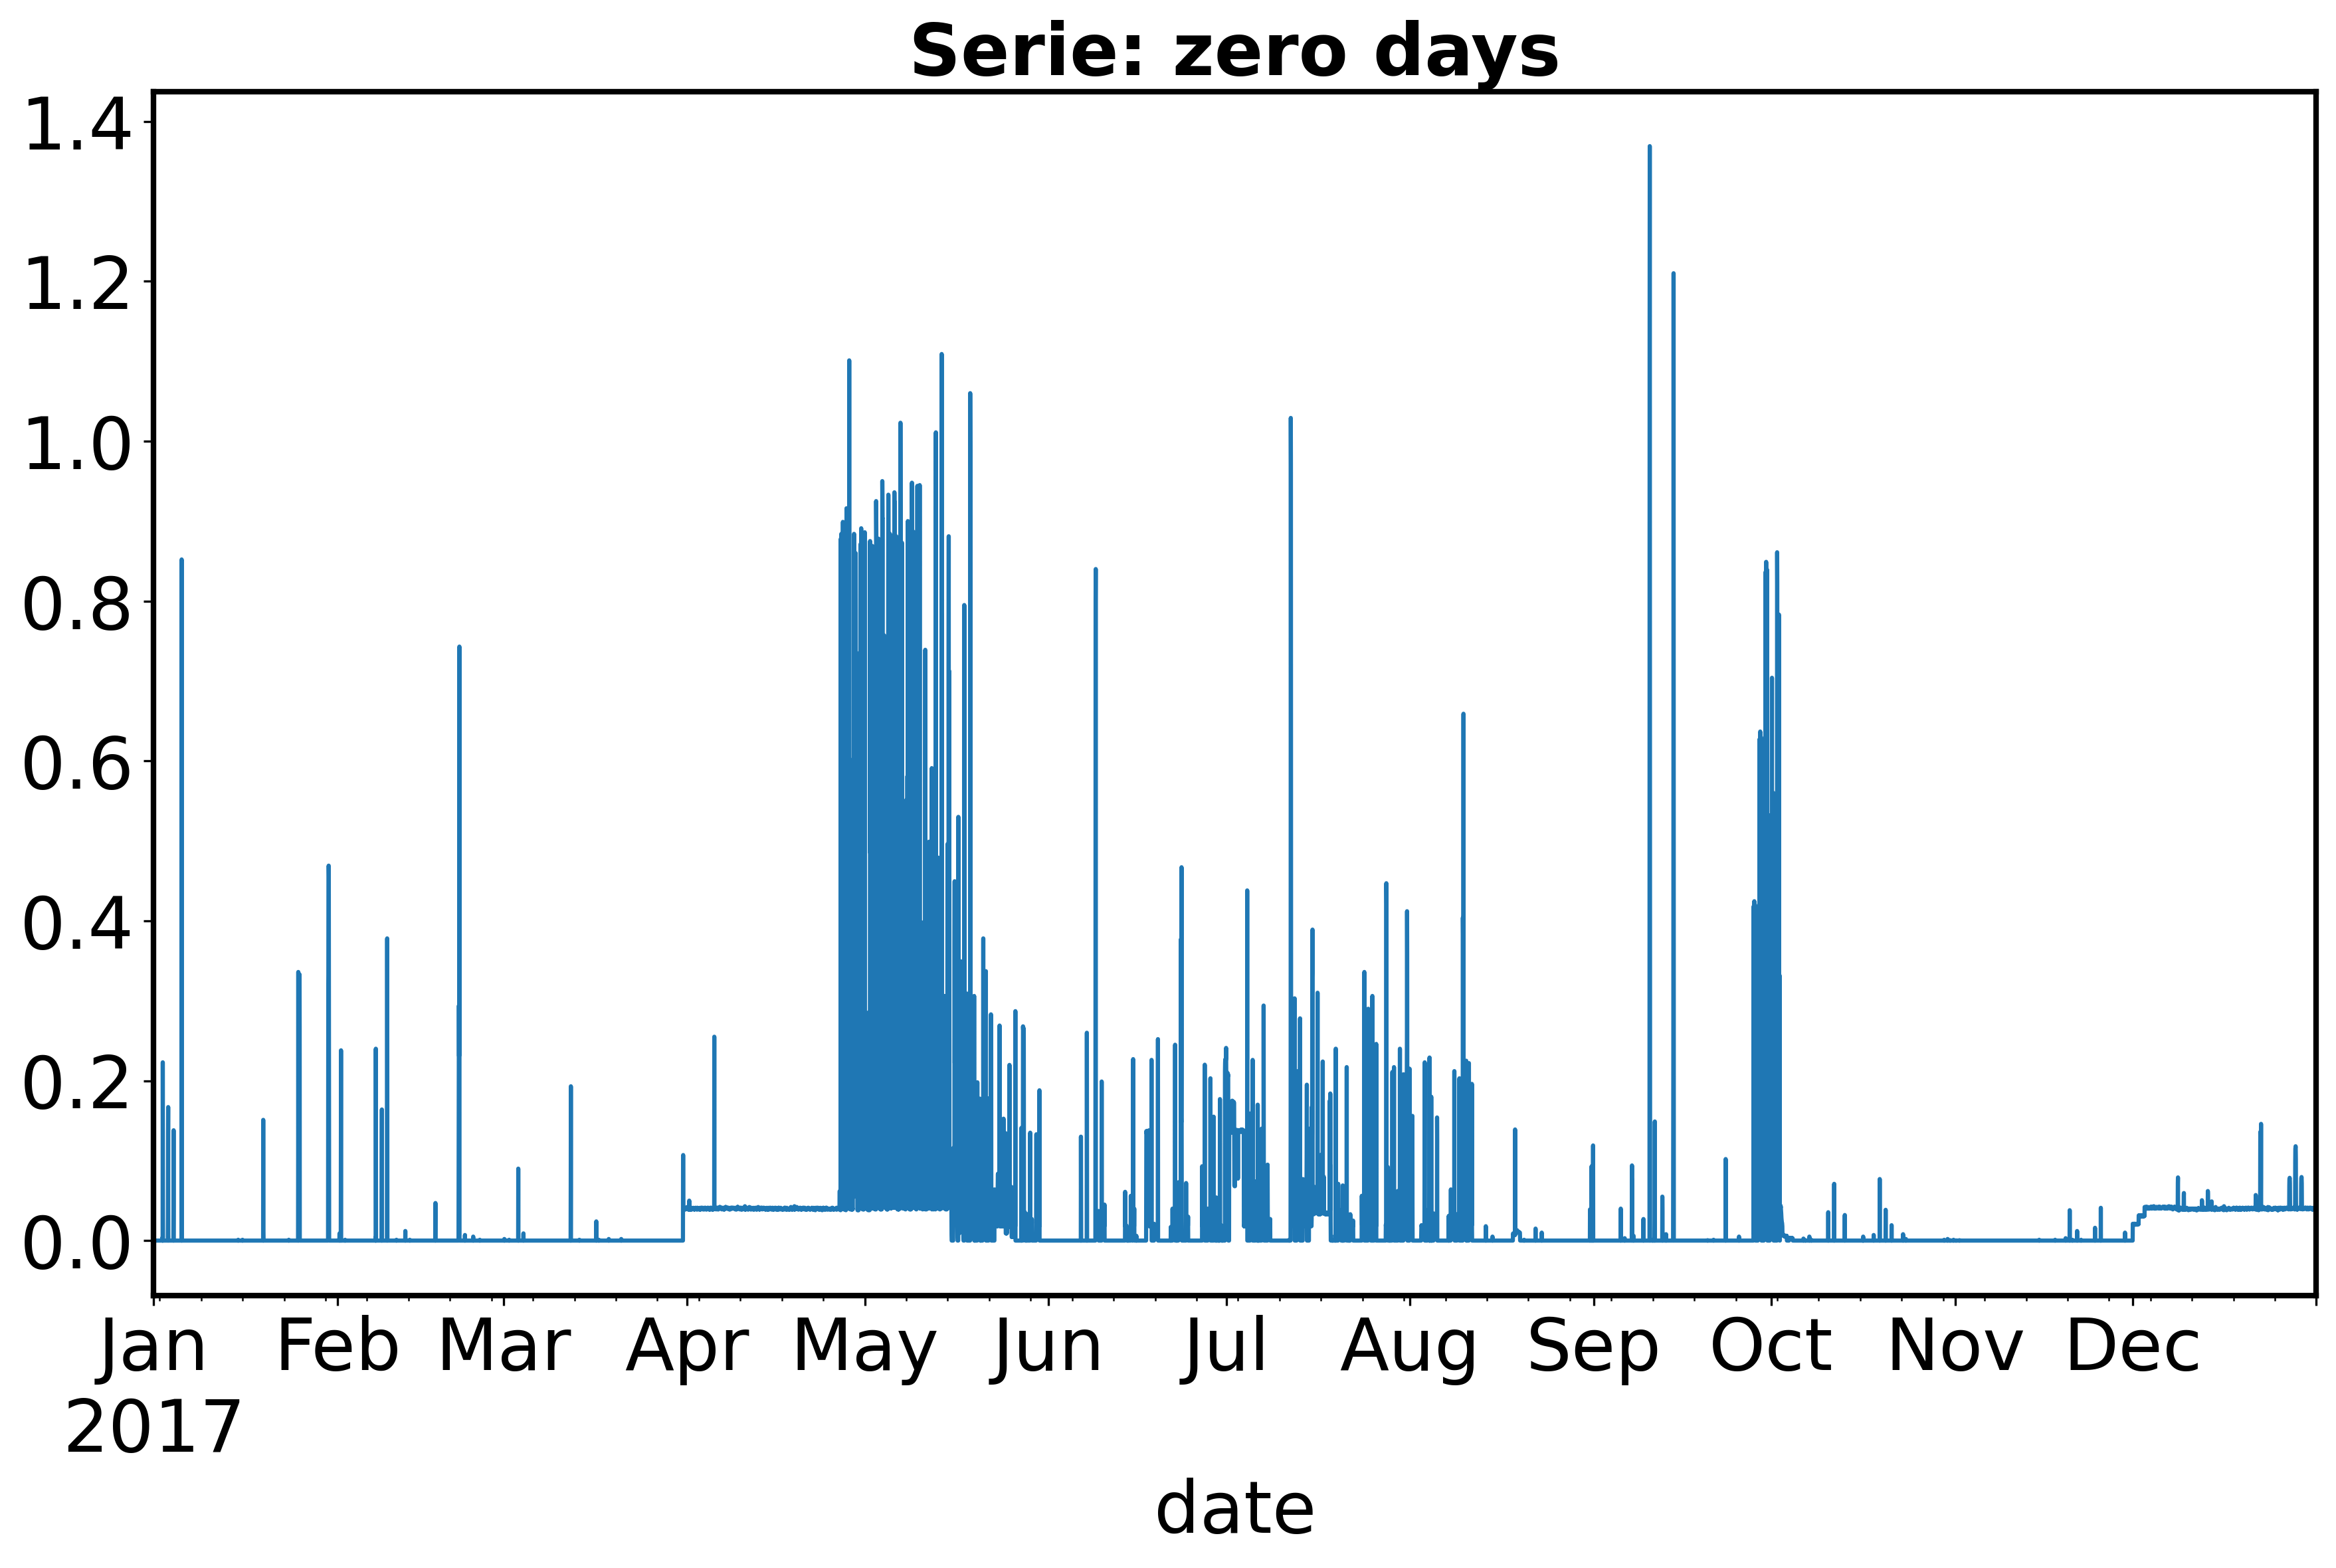
\includegraphics[width=1\linewidth]{zero_days.png}
		\caption{Serie with more than one day with zero consumption.}
	\end{subfigure}	 	
	\begin{subfigure}{0.49\textwidth}
		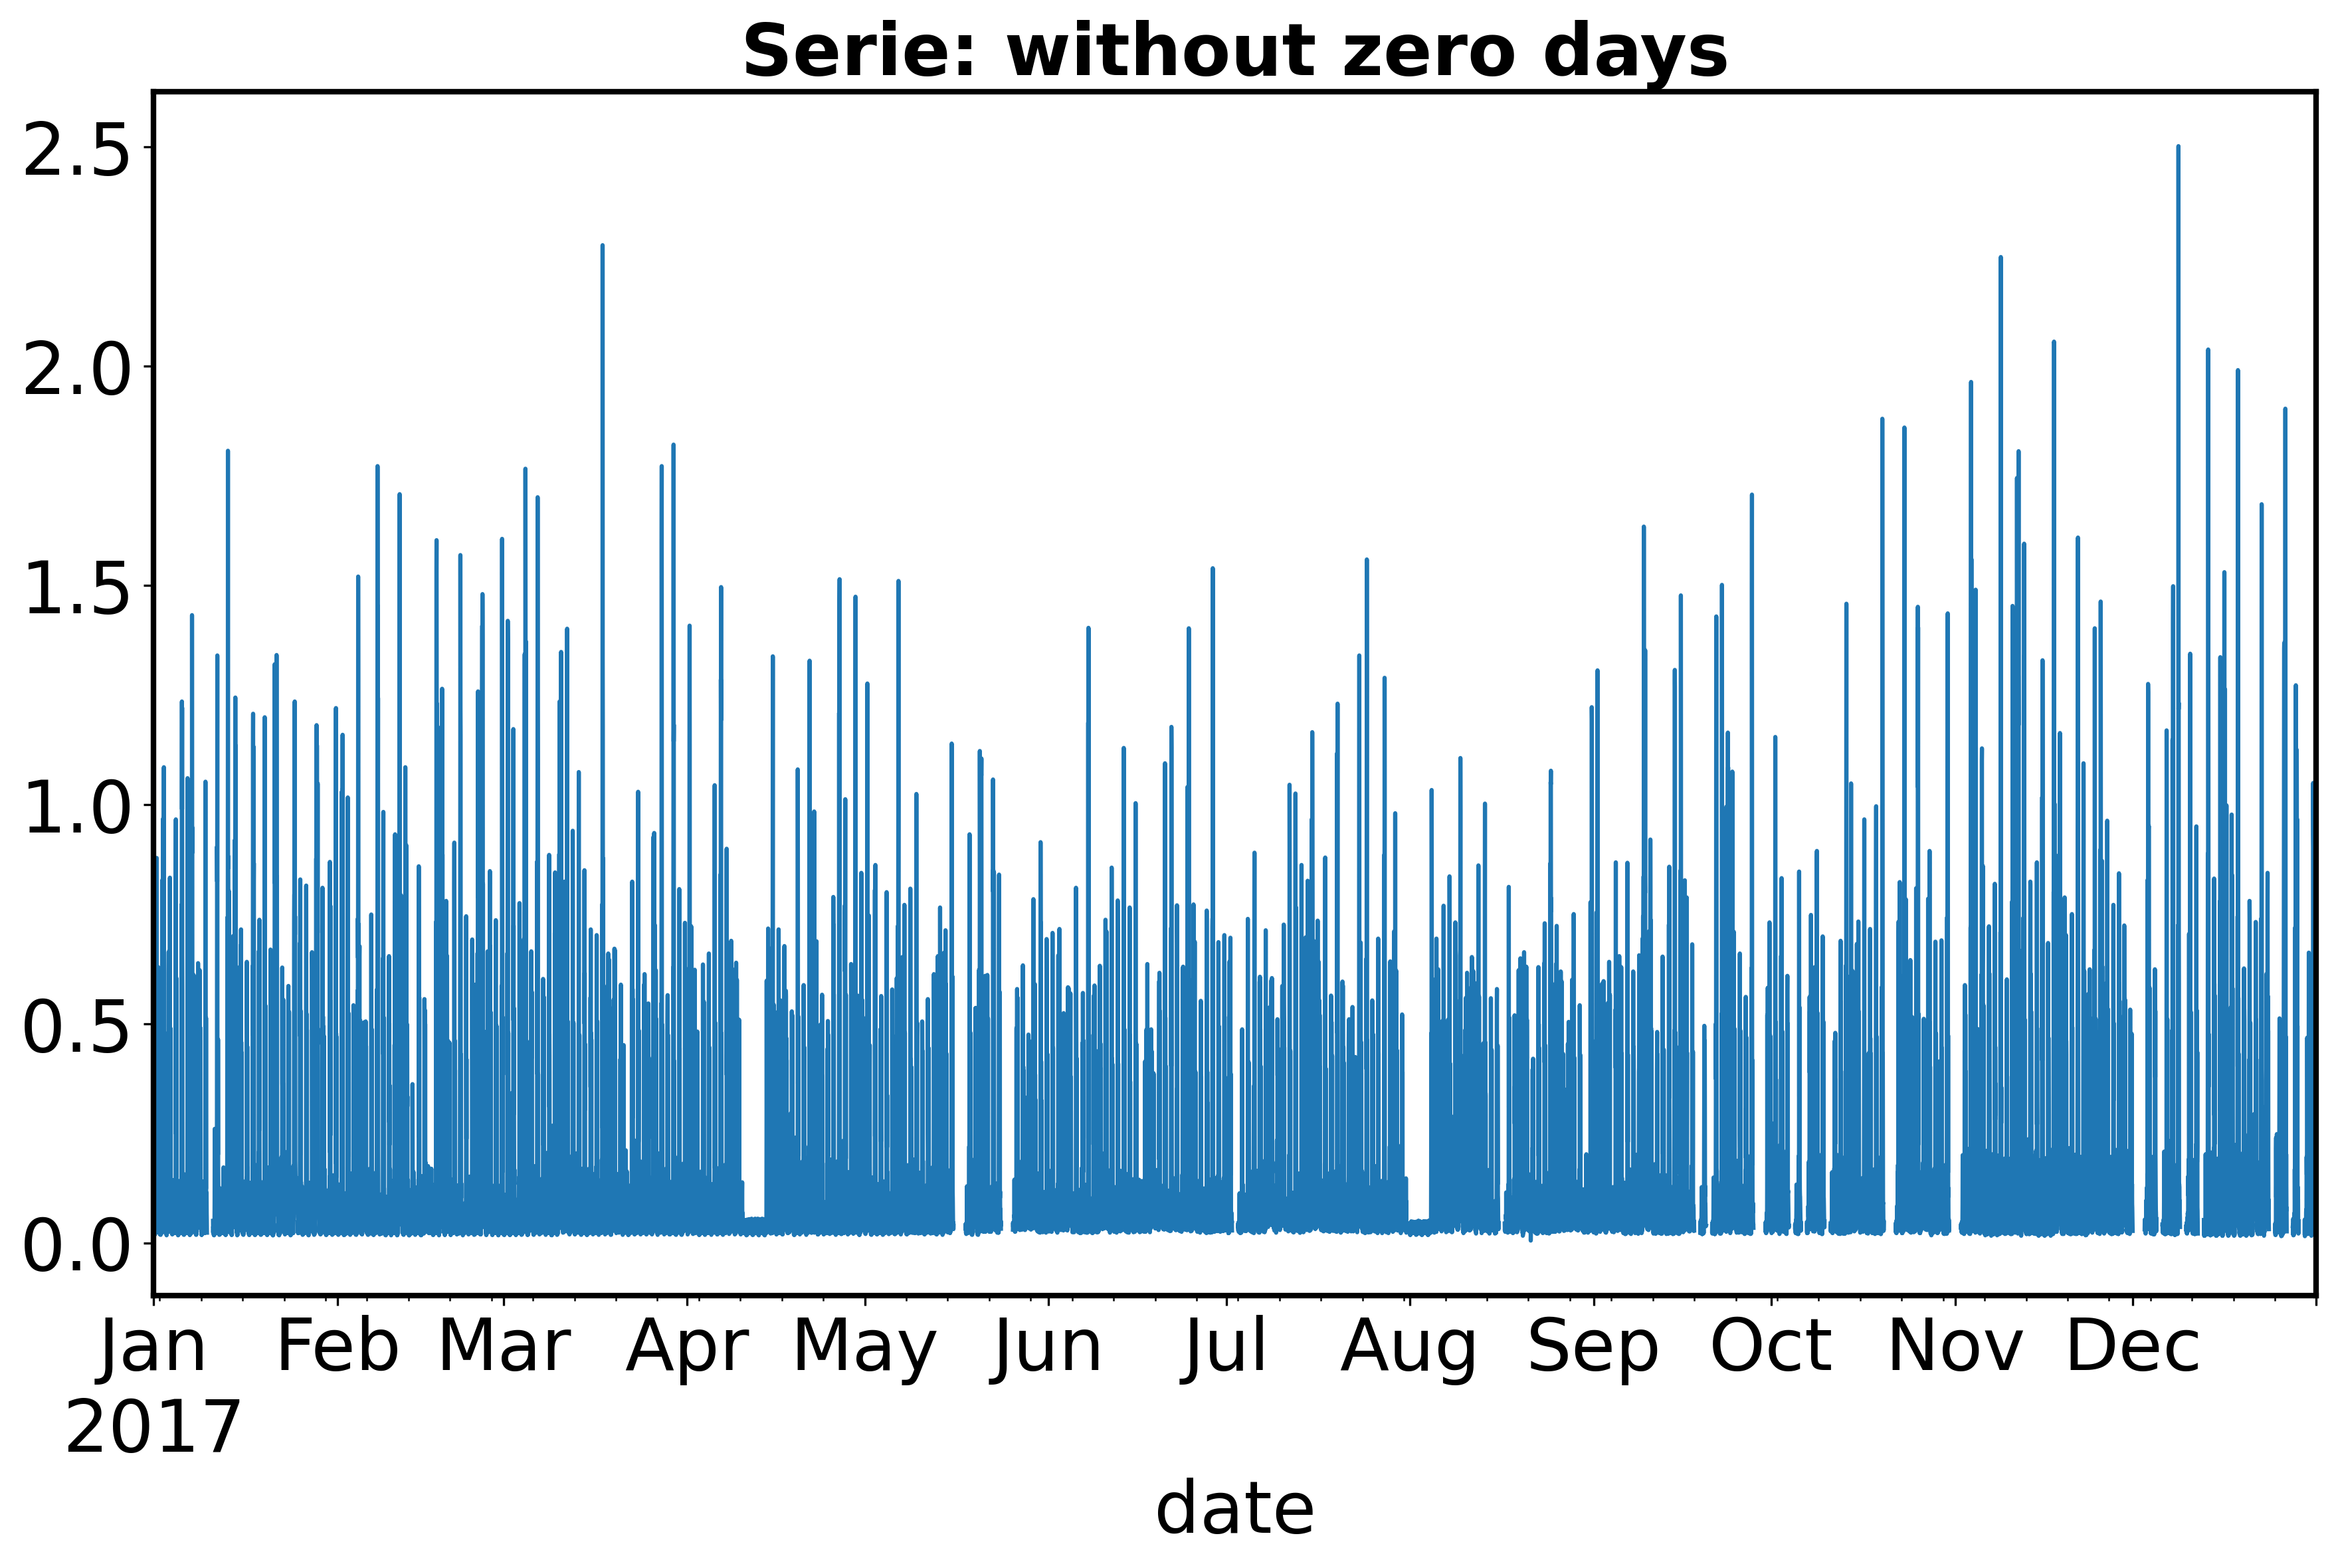
\includegraphics[width=1\linewidth]{without_zero_days.png}
		\caption{Serie $ 2 $ from Chapter \ref{cha:Forecasting the daily electricity consumption}.}
	\end{subfigure}	
	\caption{Comparison of series with and without zero load days.}
	\label{fig:zero_con}
\end{figure}

\subsection{Normalization of the data}
\label{s:Normalization of the data}
% normalize as done in ppt --> deviding by the yearly consumption.
% downside of this normalilzation that outshooters will have influence.
Normalization is necessary because while absolute consumption differs, relative patterns of human behaviour can be more similar according to \cite{Lago2020}. The goal of a forecasting model applied on an individual household is to extract the human behaviour and normalization contributes to this by avoiding the disturbance of different magnitudes in which this human pattern may occur. Every load serie is normalized based on its yearly consumption as was done by \cite{Lago2020}. The advantage of using the yearly consumption for normalization in comparison to the min-max method often used in literature, is the robustness against measurement outliers. This is important because in Section \ref{s:Data Analysis} all the 261 time series will be aggregated, which means that when a serie has only one very large outlier, the rest of its consumption values will be observed as small values in comparison with other series without a very large outlier. This is avoided when using the yearly consumption normalization where every load serie will be one at the end of the year as shown by Eq. \ref{eq:norm}. This allows for better comparison among the different series. The min-max normalization method is however used in Chapter \ref{cha:Forecasting the daily electricity consumption}, but here the series are always assessed individually

\begin{equation}\label{eq:norm}
	normalized\hspace{0.3cm} consumption_i = \frac{consumption_i}{\sum_{k=1}^{17520} consumption_k}.
\end{equation} 


\subsection{Shifts in rolling mean of load signal} \label{s:Shifts in rolling mean of load signal}
In this Section the normalized time series are assessed on fundamental changes in the load signal which can't be explained by normal human behaviour in the current household setting. A fundamental change of the load signal can be caused by an extra inhabitant or when systems are installed during the year that use a lot of electricity e.g. air-conditioning. A fundamental change is identified by looking at the maximum difference of the maximum and minimum rolling mean consumption over $ 7 $ days. Figure \ref{fig:fund_change} shows all the maximum differences between the maximum and minimum weekly rolling averages for the 261 load series. Outliers in the the maximum difference are detected as is done in a boxplot, namely from the third quartile a distance of one and a half times the interquartile range is added and values higher are considered as outliers. The red line in Figure \ref{fig:fund_change} shows when a maximum difference is considered as an outlier. Finally, the outliers which corresponds to 5 load series above the red line, are removed because they are seen as a disturbance when the load signals are aggregated in Section \ref{s:Data Analysis}. Figure \ref{fig:rolling_mean_shift} shows one of the removed load signals. 

\begin{figure}[h!]
	\centering
	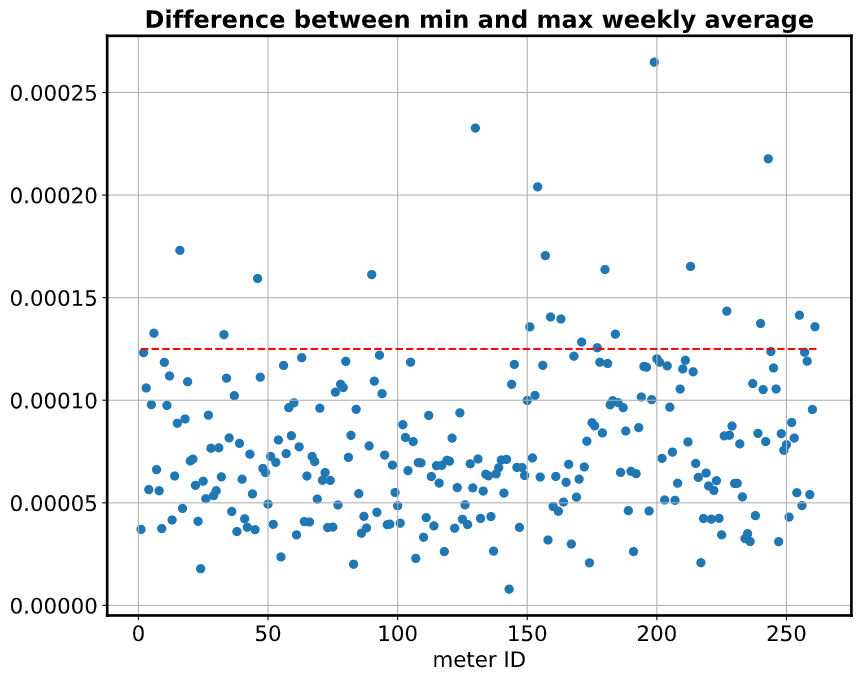
\includegraphics[width=0.8\textwidth]{fund_change.png}
	\caption{The maximum differences between the maximum and minimum weekly rolling mean for all the 261 different load signals.}
	\label{fig:fund_change}
\end{figure}


\begin{figure}[h!]
	\centering
	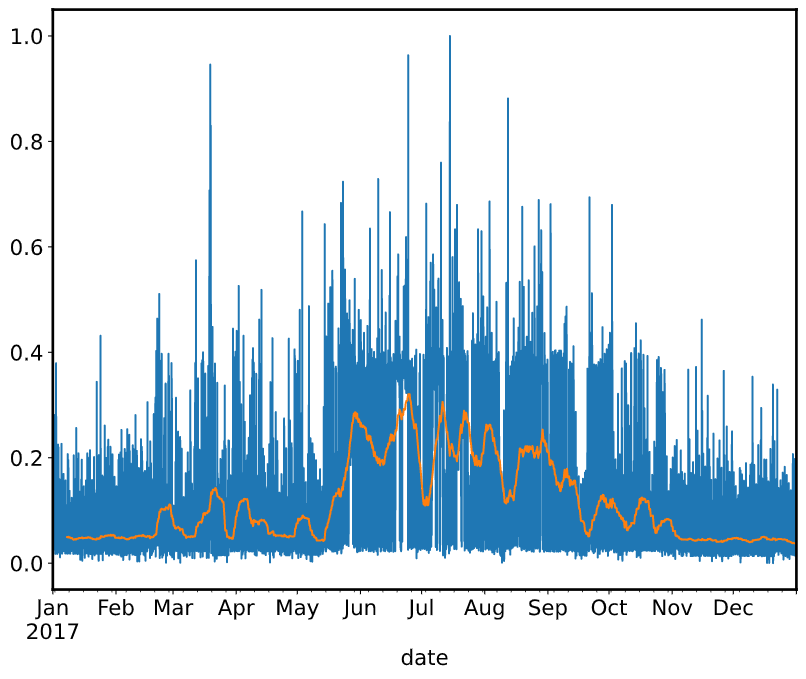
\includegraphics[width=0.8\textwidth]{fundamental_change.png}
	\caption{Removed load signal with a shift in the rolling mean.}
	\label{fig:rolling_mean_shift}
\end{figure}


\section{Data Analysis}\label{s:Data Analysis}
In this section the remaining $256$ time series are converted to a single load serie by taking the mean. The single load serie is further referenced as the mean signal. This is done to identify general characteristics of the data. Things that are going to be assessed are: seasonality, comparing electrical consumption between weekdays and weekends, impact of an holiday, the influence of the temperature and the influence of properties of the household e.g. dwelling type.


% An individual household consumption time-serie is much subdued to complex and personal decisions that cause increases or decreases of the consumption. It is hard to capture all theses effects in a single model. By aggregation of the individual time-series by taking the average, this noisy individual behaviour is mitigated. The aggregated signal is now modelled and the increase or decrease of the consumption can be explained by a small set of variables. The aggregated signal can be seen as a ``virtual distribution substation'' as discussed in \cite{Hoverstad2015}. 
 
\subsection{Seasonality}
In \cite{Hoverstad2015} it is concluded that all the forecasting algorithms that were considered, produced more accurate forecasts when they were combined with a preprocessing stage that extracted the seasonality before forecasting, compared to applying the same algorithms directly on raw data. The forecasting model is left with the task of modelling the deviation from the template consumption instead of performing a forecast out of the blue. However in \cite{Hoverstad2015} they made forecasts of an aggregated signal which had a reasonable amount of regularity which is not the case for electrical consumption forecasting of individual households. That it is not useful to extract a regular pattern is in accordance to \cite{Shi2018}, where it is explained that the use of a spectral analysis such as a wavelet analysis, that aims at separating the regular pattern from the uncertainty and the noise, is not applicable during load forecasting of individual households due to the low amount of regularity. However, the analyses of the seasonality of the mean signal is still informative to get a feeling of the general human behaviour.\\

These day and week templates are extracted from the mean signal by the use of equations \ref{eq:daily_filter} and \ref{eq:weekly_filter} that calculate respectively the average day and week indicated by a thick blue line in Figure \ref{fig:average_signals}.

\begin{equation}\label{eq:daily_filter}
	\bar{y}_i = \frac{1}{D} \sum_{d=1}^D y_{d,i}, \hspace{10mm} i \in [1,48],
\end{equation} 

\begin{equation}\label{eq:weekly_filter}
	\bar{y}_j = \frac{1}{W} \sum_{w=1}^W y_{w,j}, \hspace{10mm}  j \in [1,336].
\end{equation} 

 $ D $ and $ W $ give respectively the amount of days and weeks in the year 2017. $\bar{y}_i$ and $\bar{y}_j$ give the consumption of half an hour, averaged over respectively all days and weeks. In Figure \ref{fig:average_signals} a clear consumption peak can be seen after midnight. This is due to heat storage systems that use electricity in the hours of low tariff and that release heat during high electricity tariffs. The daily seasonality shows a small peak in the load around 7 am and a bigger one around 6 pm. In the weekly seasonality it can be seen that all the peaks at 6 pm are of the same height but the smaller peak is different depending if it is a weekday or weekend as will be further explained in Section \ref{s:Comparing weekdays with weekends}. 

\begin{figure}[h!]
	\begin{subfigure}{1.0\textwidth}
		\centering
		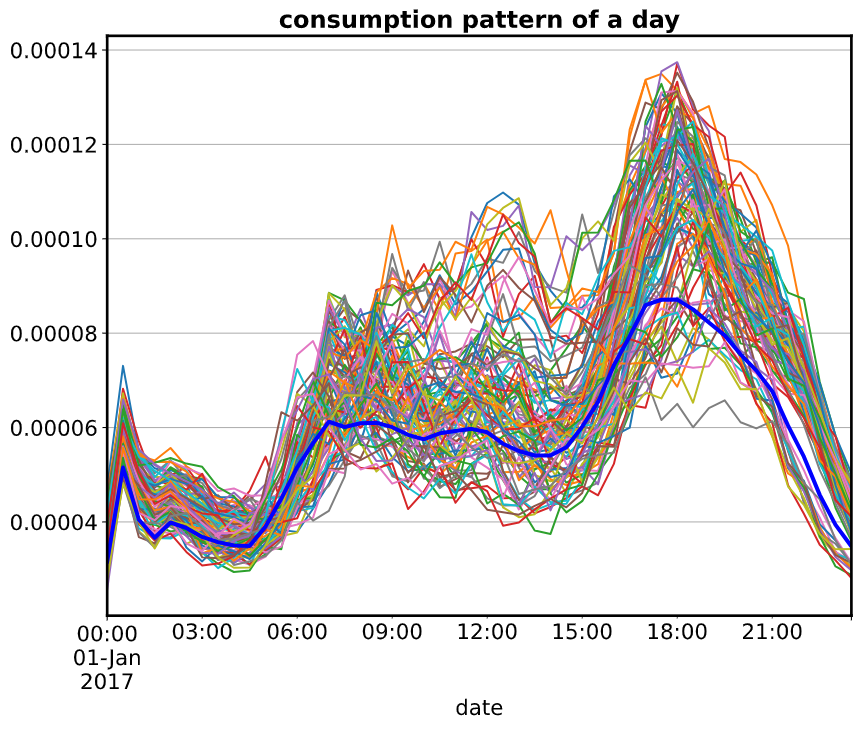
\includegraphics[width=0.7\linewidth]{daily_filter.png}
		\caption{Daily seasonality}
	\end{subfigure}	 	
	\begin{subfigure}{1.0\textwidth}
		\centering
		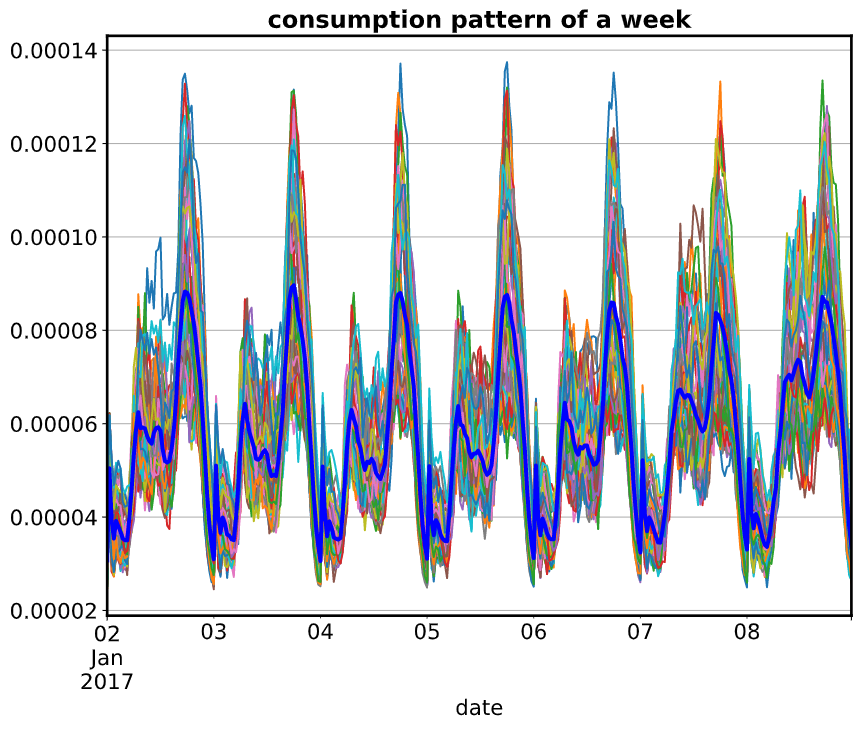
\includegraphics[width=0.7\linewidth]{weekly_filter.png}
		\caption{Weekly seasonality}
	\end{subfigure}	
	\caption{The seasonality of the electrical load during the year 2017. The blue line indicates the average load signal. }
	\label{fig:average_signals}
\end{figure}


% plot the moving average of the year. Clearly see the impact of the summer and winter.
% This is a trend that can be taken into account when predicting.



\subsection{Comparing weekdays with weekends} \label{s:Comparing weekdays with weekends}
Weekdays and weekends are compared with the help of Figure \ref{fig:average_signals}. It is clear that the consumption of the average business day is similar to a weekend day considering the time of three two peaks each day. There is a morning peak around 7 am, an evening peak around 6pm and a peak after midnight. However, in the weekends, the morning peaks seems to be a little higher and decreases less. The effect can be seen during both weekend days, but is most visible on the Sundays. To prove previous statements, the similarity is assessed by calculating the normalized MAE is calculated for the hourly difference of each combination of 2 days of the week. Normalization is done by dividing the different MAE's by the biggest MAE calculated. Figure \ref{fig:similarity_weekdays} shows in blue and orange the error of combinations between business days or weekend days and in green the error of combinations between a business day and weekend day. It can be clearly seen that when a business day and weekend day are combined (green) the error is larger and thus more dissimilar. The left cluster of dots corresponds to a Saturday that is combined with a weekday and the right cluster corresponds to a Sunday combined with a weekday. It can be noticed that Saturdays are more similar to a business day than a Sundays. 

\begin{figure}[h!]
	\centering
	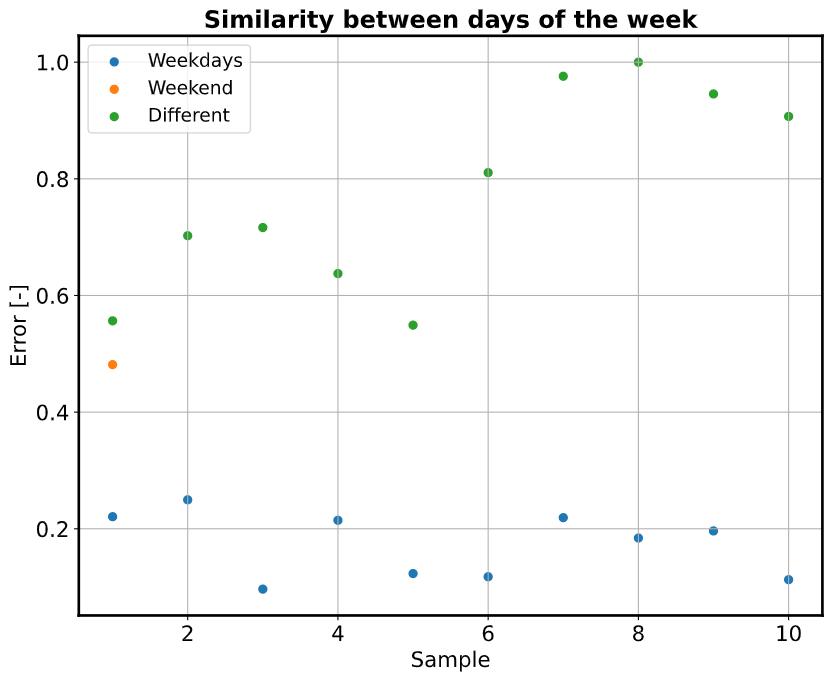
\includegraphics[width=0.8\textwidth]{similarity_weekdays.png}
	\caption{Error between different pairs of weekdays.}
	\label{fig:similarity_weekdays}
\end{figure}

\subsection{Impact of bank holidays}\label{s:Impact of holidays}
% important that look at holidays in the UK. In paper \cite{Hoverstad2015} all the holydays are subsitued by the same day the next week and the previous week. It is possible to look at all the holidays, normalize them concerning temperature and try to get a seasonality model. 
In order to look at the impact of a bank holiday, all the holidays of the English and Welsh calendar are identified for the year $ 2017 $. For each of the $ 8 $ bank holidays a corresponding business day is selected with an in euclidean distance as close as possible average temperature of the day. Therefore, mitigating the temperature influence. Note that each of the 8 holidays or business days are from the mean signal and they therefore are already averaged over 256 load signals. The 8 bank holidays and business days are averaged to obtain Figure \ref{fig:bvsh}. It is observed that a bank holiday behaves similarly to a weekend day which means a higher morning peak that decreases less. Figure \ref{fig:sim_weekdays} illustrates the similarity between a holiday and the days of the week. The error is calculated as the MAE of the hourly difference between the average day of the week and holiday. It can be seen that a bank holiday behaves most similarly to a Sunday.

\begin{figure}[h!]
	\centering
	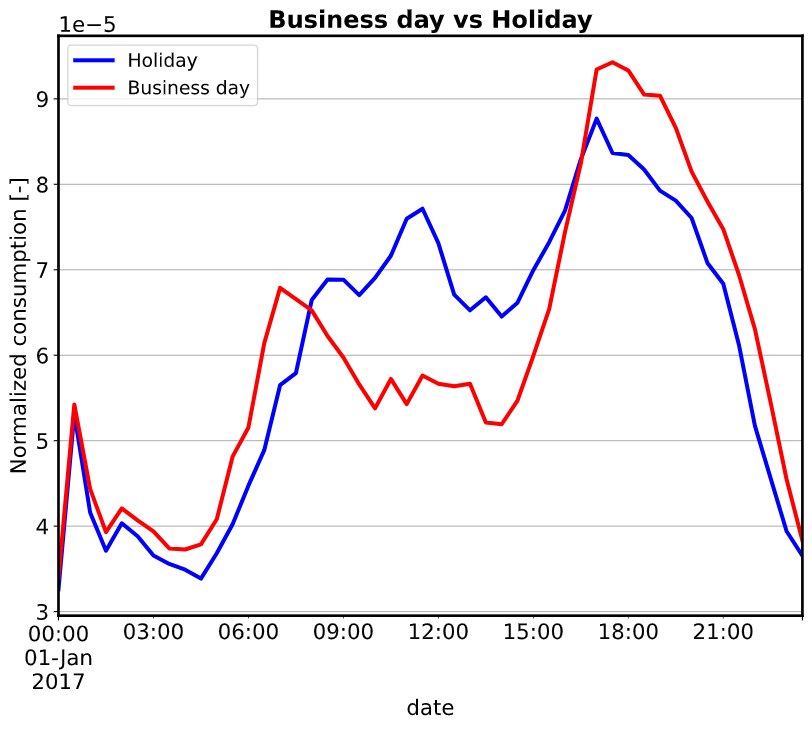
\includegraphics[width=0.6\textwidth]{bvsh.png}
	\caption{Comparison between bank holiday and business day electrical consumption.}
	\label{fig:bvsh}
\end{figure}

\begin{figure}[h!]
	\centering
	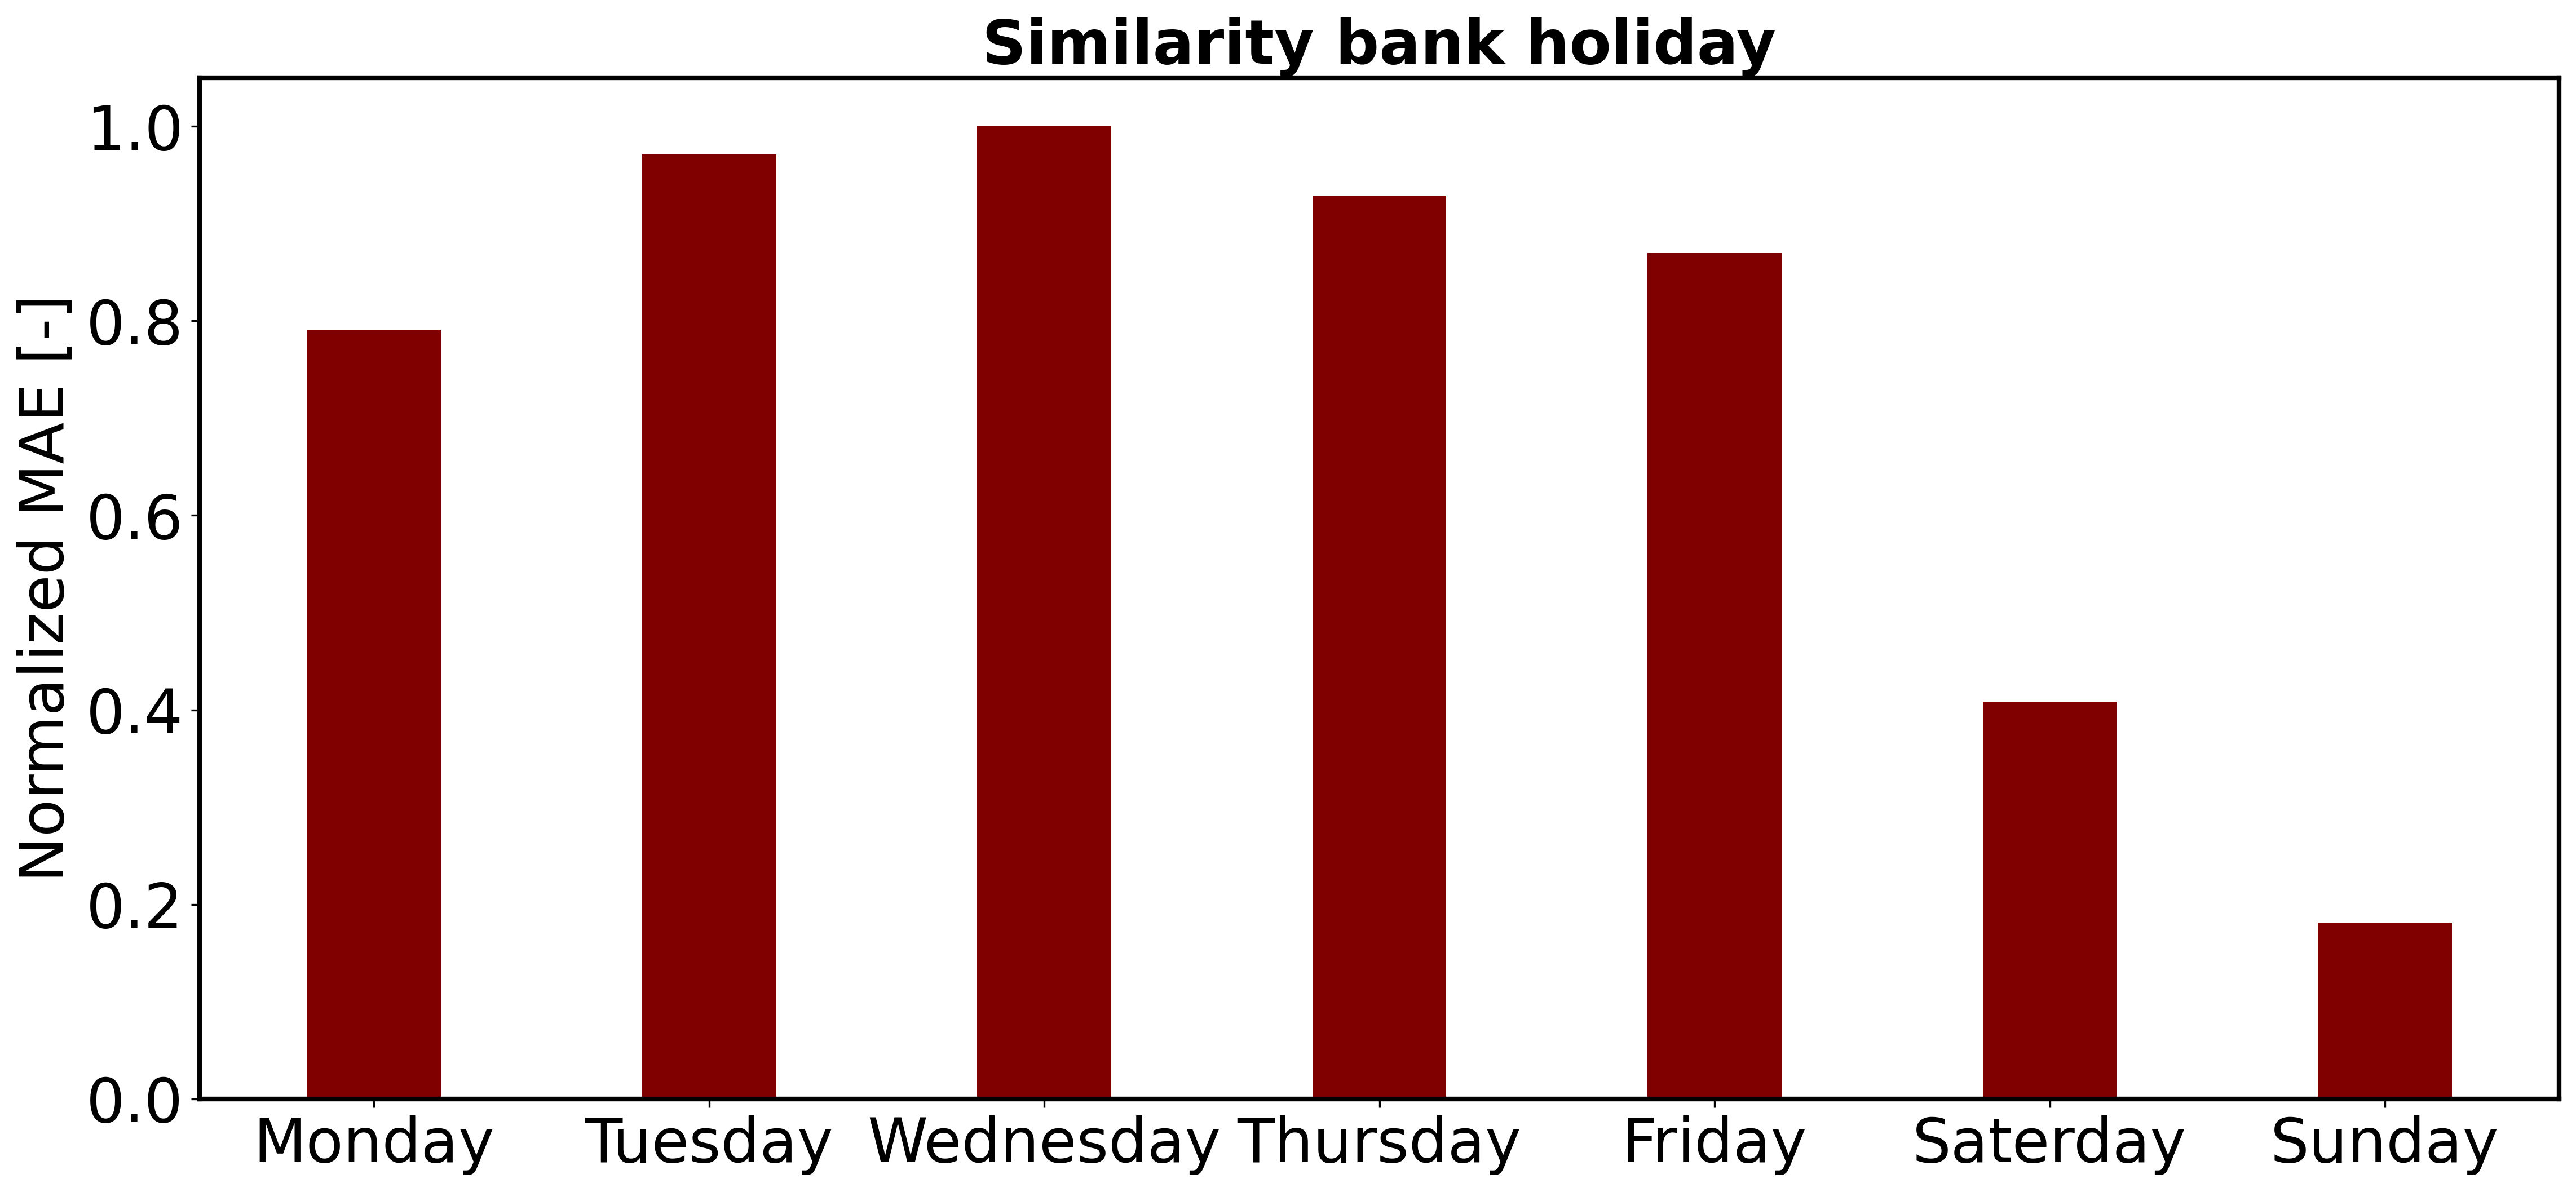
\includegraphics[width=1.0\textwidth]{similarity.png}
	\caption{Error between a bank holiday and other days of the week.}
	\label{fig:sim_weekdays}
\end{figure}


\subsection{Influence of temperature}
% notes on correlation see OneNote.
% use the correlations. https://realpython.com/numpy-scipy-pandas-correlation-python/
% resample the consumption to daily and then apply some of the correlation techniques. 
In this section the correlation between the temperature and the electricity consumption is discussed.\\


\textbf{Pearson correlation}\\
The Pearson correlation is a measure of the linear dependency between two variables, based on the covariance. A Pearson correlation value gives information concerning the magnitude of the association and the corresponding direction of it. A Pearson value of $ 1 $ and $ -1 $ gives respectively a perfect positive and negative linear relation between the variables. A value of zero, corresponds to independent behaviour. The following formula gives the Pearson correlation

\begin{equation}\label{eq:pearson}
	\rho_{X,Y} = \frac{cov(X,Y)}{\sigma_x\sigma_y}.
\end{equation}

Assumptions concerning the Pearson correlation are that samples used for the correlation should be independently drawn, coming in pairs, following homoscedasticity and there are no outliers. Outliers are especially undesirable when there are not a lot of samples. The variables should be normally distributed, linearly related to each other and be continuous. A normal distribution is necessary otherwise the assumption that a distribution can be described by a mean and variance is violated. The samples used for the correlation are generated by calculating the daily consumptions matched with the daily average temperature of the mean signal. Homoscedasticity is important because Eq. \ref{eq:pearson} assumes that $ \sigma_x $ and $ \sigma_y $ are constant values. The homoscedasticity assumption is validated by making use of Figure \ref{fig:pearson}.

\begin{figure}[h]
	\centering
	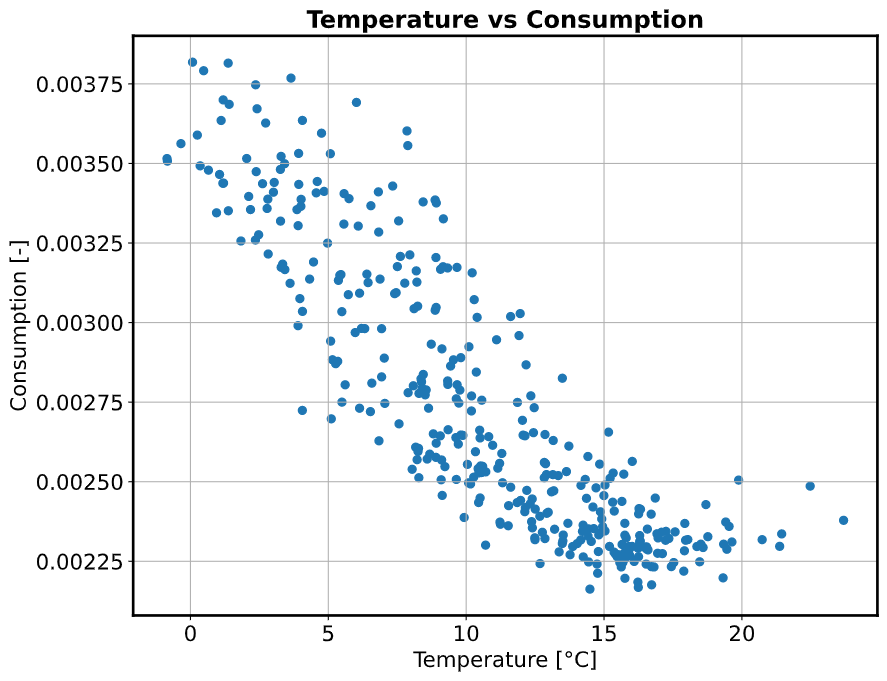
\includegraphics[width=0.8\textwidth]{pearson.png}
	\caption{Relation between normalized daily consumption and daily temperature.}
	\label{fig:pearson}
\end{figure}

This figure shows the classic cone-shaped pattern of heteroscedasticity. On days when it is warm there is more similar human behaviour in lowering the electricity consumption. However, on colder days the variation in consumption is higher, which means that homoscedasticity is not perfectly fulfilled. This is a logical result because when it is cold there can be a lot of variation in what extent electricity is used for heating, while when it is warm everybody is likely to turn of the heating. Because the assumptions of the Pearson correlation are not all met, care should be taken with the output. Applying the Pearson correlation on Figure \ref{fig:pearson} gives a correlation value of $ -0.87 $. This means there is a good linear, decreasing relation.\\


\textbf{Spearman correlation}\\
The Spearman correlation is a rank correlation. A sample consists out of a daily consumption value with a corresponding average temperature value.
The consumption and temperature values belonging to a sample are each compared with respect to all the consumption and temperature values and an ordering is retrieved for both values. When the ordering of both variables in a sample is similar, correlation is strong and positive. If the ordering is reversed, correlation is strong and negative. There is a perfect positive ordering if a larger consumption always corresponds to a higher temperature. Notice that for a perfect ordering, no linear relation of the variables is necessary. The Spearman correlation coefficient is calculated using Eq. \ref{eq:pearson}, but replaces the values of the variables by the rank of the variables in the a sample.\\

In order to use the Spearman correlation data has to be ordinal, which means that it can be ordered. The Spearman correlation gives information about the monotonicity relation between the variables. $ \rho = 1 $ corresponds to a monotonically increasing relation.\\

Applying the Spearman correlation  gives a correlation value of $ -0.89$, which means there is a large negative monotone relation. This means if the temperature is higher, consumption is likely to be lower and the . Identically, if the temperature is lower it is likely that the consumption will be higher and vice versa. This confirms the conclusions from the Pearson correlation.\\

\textbf{Kendal correlation}\\
The Kendal correlation is also a rank correlation. It is looked how many samples are concordant, discordant or neither when each combination of 2 samples are compared with each other. A concordant pair means that when the consumption value of sample 1 is higher than the consumption value of sample 2, this must also be the case for the temperature values. A discordant pair means that when the consumption value of sample 1 is higher than the consumption value of sample 2, this should be not the case for the temperature. Neither can occur when consumption values or temperature values are equal for the 2 samples. When a Kendal correlation of 1 is retrieved, this means that all samples are concordant and only $ n^+ $ differs from zero. This automatically imposes monotonicity which means that when a consumption value is increased, also the temperature value must be increased. Equation \ref{eq:kendall} gives the equation to calculate the Kendal correlation coefficient. Applying the Kendal correlation  gives a correlation value of $ -0.67$, which again confirms the conclusions from the Pearson correlation.\\

\begin{equation}\label{eq:kendall}
	\tau = \frac{n^+-n^-}{\sqrt{(n^++n^-+n^x)(n^++n^-+n^y)}}
\end{equation}
\begin{itemize}
	\item $ n^+ $ is the number of concordant pairs
	\item $ n^- $ is the number of discordant pairs
	\item $ n^x $ is the number of ties only in x
	\item $ n^y $ is the number of ties only in y
	\item concordant $\rightarrow $ $ (x_i > x_j ) $ and $ (y_i > y_j ) $ or $ (x_i < x_j ) $ and $ (y_i < y_j ) $
	\item discordant $\rightarrow $ $ (x_i > x_j ) $ and $ (y_i < y_j ) $ or $ (x_i < x_j ) $ and $ (y_i > y_j ) $
	\item neither $\rightarrow $ $ (x_i = x_j ) $ or $ (y_i = y_j ) $
	\item if both $ (x_i = x_j ) $ and $ (y_i = y_j ) $ $\rightarrow $ not included in either $ n^x $ or $ n^y $
\end{itemize}



% There is a clear dependency between temperature and electricity consumption, which means that electricity is used for heating.  

\subsection{Identification of the influence of household attributes} \label{s:Identification of driving attributes}
In this section the influence of different attributes of the households on the load signals is investigated. Instead of the mean signal every smart meter of the total of 3248 meters with additional information, is used during the analysis. This means that also load series are included that don't have measurements for the full year as was discussed in Section \ref{s:missing_data}. Because all load signals have measurements for the month December, the total consumption during December is used in the analysis. Missing values during December are imputed according to the Average neighbours method.\\
It is observed that only for the dwelling type and the amount of bedrooms, there is a higher response in the questionnaire. Respectively, 1702 and 1859 answers are obtained in comparison to the rest of the questions were the amount of collected answers varies between 69 and 78. sometimes, the answers are not well distributed over the different options, for example when assessing heating fuel there are only three answers registrated for using electricity in comparison to 69 answers that are registrated for using gas. An overview of the amount of answers per household attribute, can be seen in Table \ref{tab:attributes}. Because of the low sample sizes of the attributes different from dwelling type and number of bedrooms, care should be taken with the outcomes of the stochastic analysis.\\
Figure \ref{fig:boxplots} shows boxplots of the collected data concerning the dwelling type and the amount of bedrooms. According to the mean and median values of the different dwelling types, the order in monthly consumption is: Flat < Bungalow < Semi detached < Terraced < Detached. It was noted that there were a lot of outliers in the consumption values of a detached house. A ``real'' house also tends to have a higher monthly consumptions than a flat or bungalow. Next, it is observed that when a housing unit has more bedrooms, also the monthly consumption is larger. This is a logical result, because it is likely that when the number of bedrooms is larger, the house is larger which means that it requires more electrical heating when used and it can store more electrical appliances. Conclusions drawn for the other attributes are summarized below.

\begin{figure}[h!]
	\begin{subfigure}{1.0\textwidth}
		\centering
		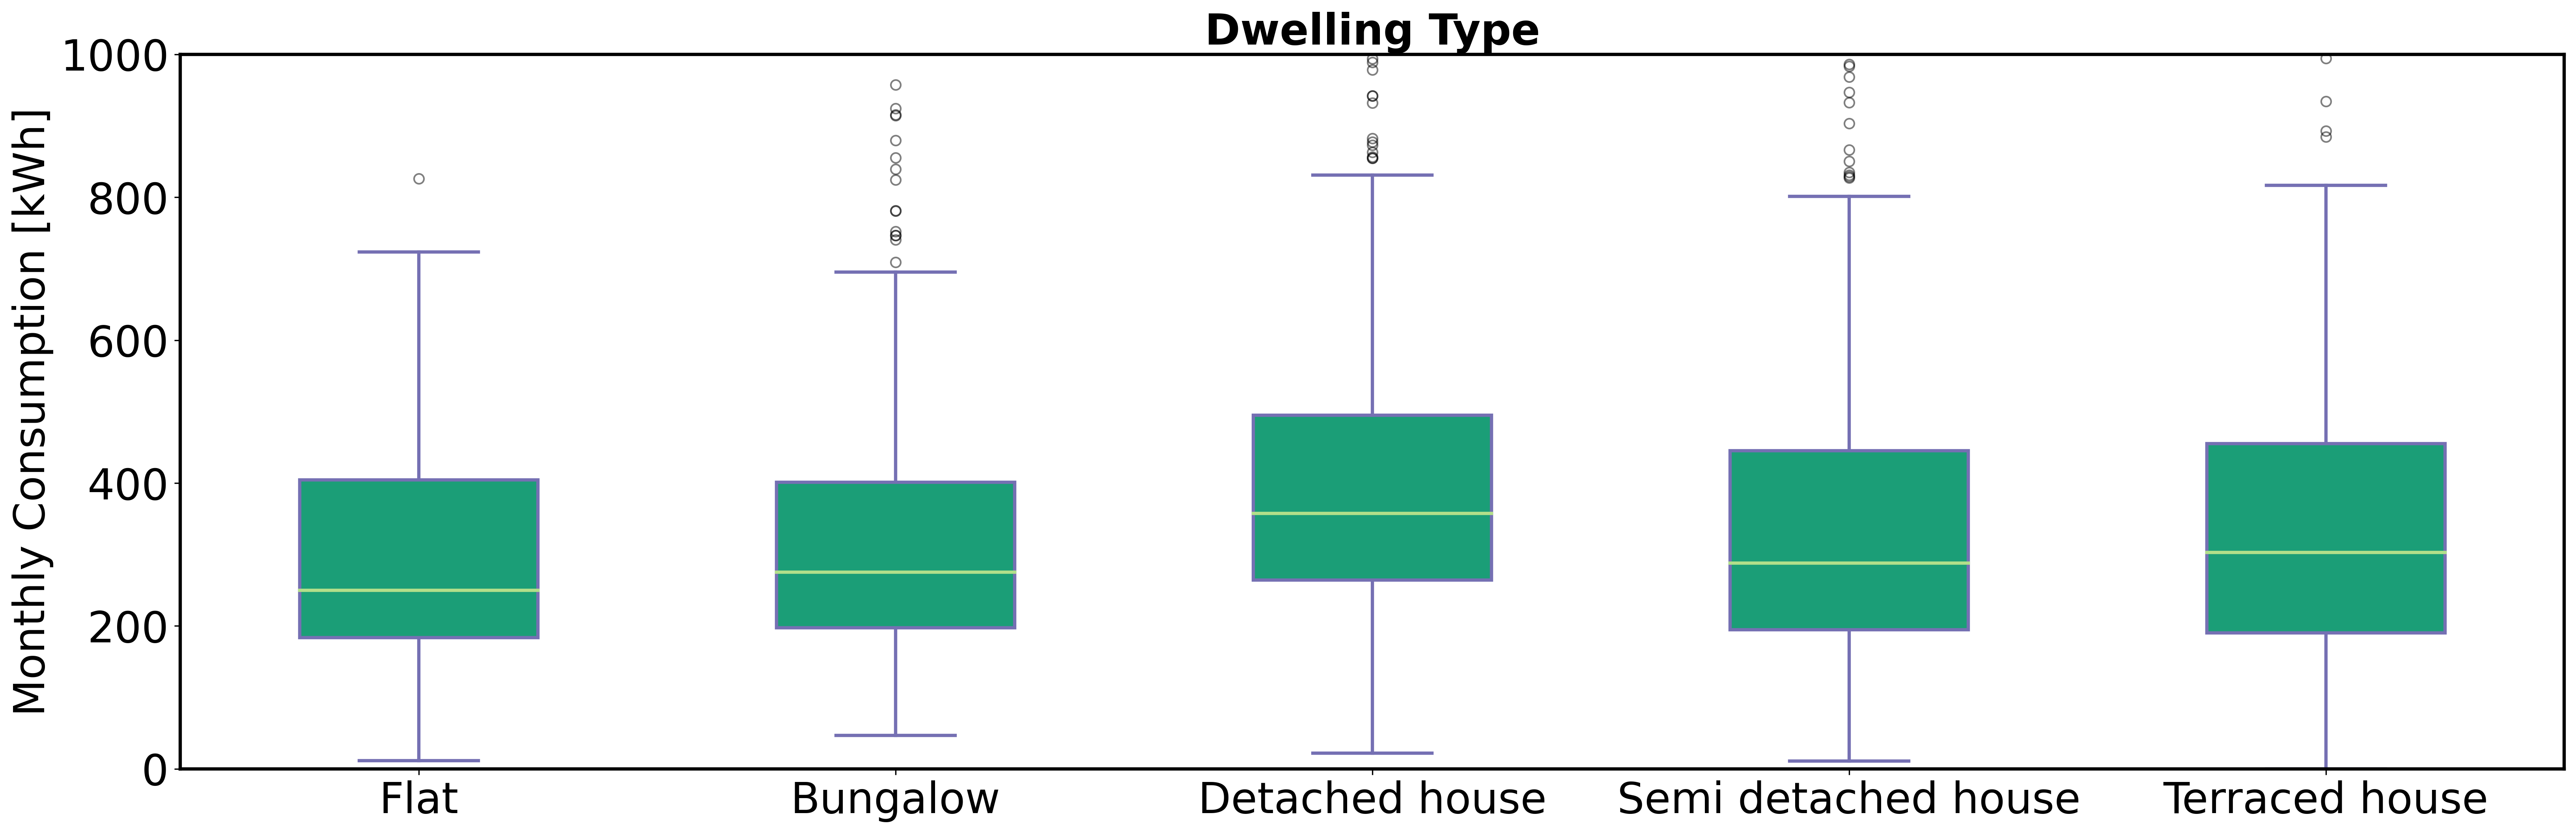
\includegraphics[width=1.0\linewidth]{dwelling_type.png}
		\caption{Dwelling type}
	\end{subfigure}	 	
	\begin{subfigure}{1.0\textwidth}
		\centering
		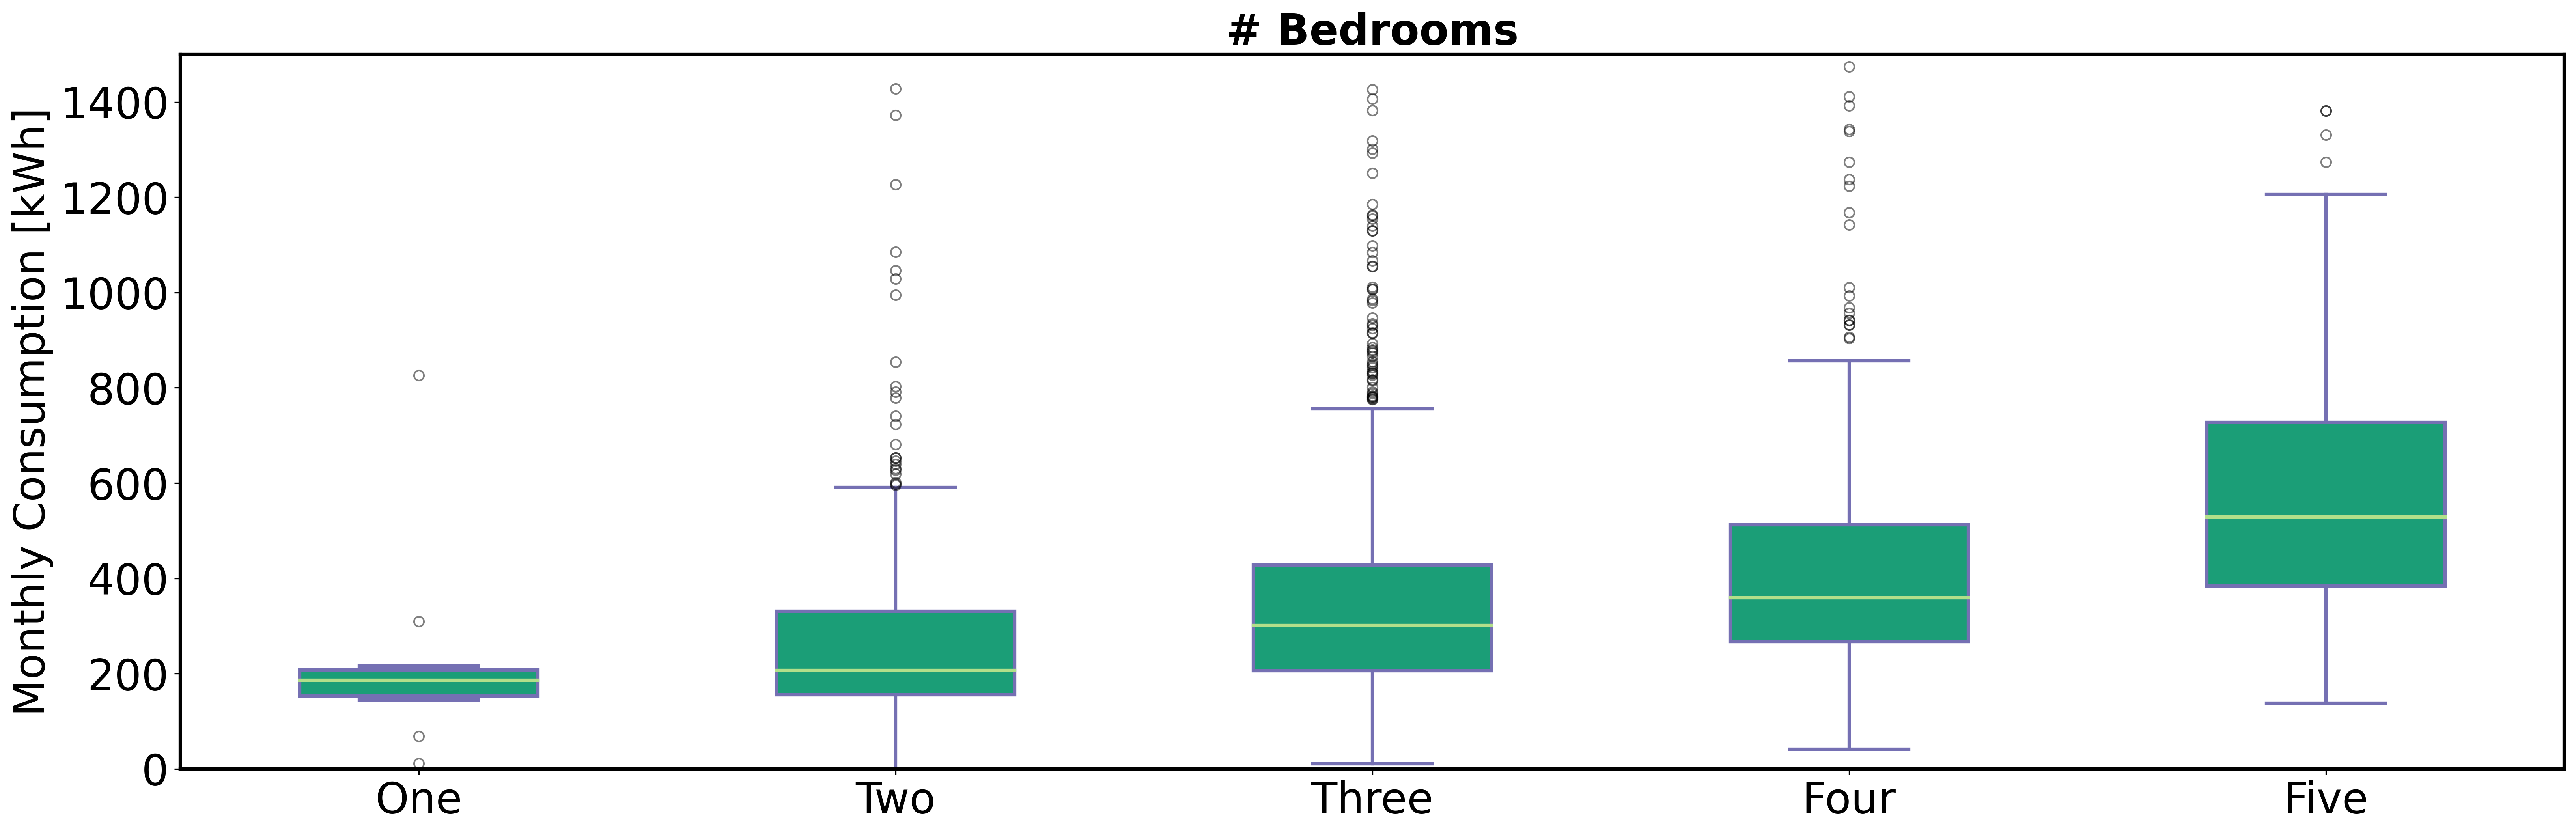
\includegraphics[width=1.0\linewidth]{num_bedrooms.png}
		\caption{Number of bedrooms}
	\end{subfigure}	
	\caption{Influence of the dwelling type (sample size: 1702) and number of bedrooms (sample size: 1859). }
	\label{fig:boxplots}
\end{figure}

%Similar as was done in Figure \ref{fig:bp_dwellingtype} is also done for the other characteristics of the smart meters. The conclusions are listed below. As can be seen in Table \ref{tab:attributes}, some characteristics have not much data or the data is not much distribute over the different options of a characteristic. If this is the case, no reliable conclusions could be drawn. \textbf{Add concrete numbers!!}

\begin{itemize}
	\item More inhabitants means more monthly consumption
	\item 88$ \% $  of the households use gas as heating fuel
	\item 81$ \% $  of all houses use gas as hot water fuel
	\item When the boiler age is categorized as old, the median of the monthly consumption is 30$ \% $ higher with respect to the median of a new boiler
	\item 91$\% $ of the lofts are insulated
	\item 72$ \% $ of the walls are insulated
	\item 76$ \% $ heats till a temperature between $ 18 $ and $ 20  $ degrees
	\item 66$ \% $ has an efficient lighting percentage between $ 75\% $ and $ 100\% $	
\end{itemize}



\section{Conclusion}
During this chapter the exploratory data analysis of the data retrieved form the IEEE-CIS technical challenge on energy prediction from smart data, is conducted. First, the data was described by giving its most important features and displaying the amount of NaN values. It was found that there are 261 load signals with a full year of measurements.  Next, preprocessing of the data was done by discussing the imputation of the missing values, the identification of zero days, normalization and shifts in the rolling mean of the load signal. Thereafter, the data analysis followed were an aggregated load signal was assessed and seasonality, weekdays versus weekend days, impact of bank holidays and the influence of the temperature were explained. Finally, the influence of household attributes was discussed. 



%Please don't abuse enumerations: short enumerations shouldn't use
%``\verb|itemize|'' or ``\texttt{enumerate}'' environments.
%So \emph{never write}: 
%\begin{quote}
%	The Eiffel tower has three floors:
%	\begin{itemize}
%		\item the first one;
%		\item the second one;
%		\item the third one.
%	\end{itemize}
%\end{quote}
%But write:
%\begin{quote}
%	The Eiffel tower has three floors: the first one, the second one, and the
%	third one.
%\end{quote}

%%% Local Variables: 
%%% mode: latex
%%% TeX-master: "thesis"
%%% End: 
